\subsection{Documentation for alamPREPROCESSOR}
\label{subsec:doc_preproc}
The documentation section for the alamPREPROCESSOR discusses the currently implemented features, 
as well as a guide to the file directories to manage these files as effectively as possible for 
any future updates, maintenance work, and testing required.

\subsubsection{alamPREPROCESSOR Features}
\label{subsubsec:alamPREPROCESSOR_features}
The current features implemented in the alamPREPROCESSOR are as follows:
\begin{itemize}
    \item[(a)] The Data Collector Module (DCM) was integrated into the alamPREPROCESSOR 
    to allow the alamSYS to collect end-of-day historical data from the various stocks on 
    the Philippine Stock Exchange (including the PSEI). EODHD data is collected using the web API.
    \item[(b)] The Data Processor Module (DPM) was built into the alamPREPROCESSOR to enable the 
    alamSYS to perform the following tasks:
    \begin{itemize}
        \item[1.] Apply DMD-LSTM to each stock dataset.
        \item[2.] Create a list of stocks to buy and sell by applying the ALMACD to the last 200 
        days of actual stock data and the five predicted data points from the DMD-LSTM model; and
        \item[3.] Update the database with new information about which stocks to buy or sell.
    \end{itemize}
    \item[(c)] The alamPREPROCESSOR handles items (a) and (b) automatically. 
    This means that they are set to run at a specific time, which is 6 p.m. every Monday through Friday. 
    Some errors are also handled automatically if they are internally related, which means they are not affected 
    by external factors such as a slow and unstable internet connection, a downtime in the EODHD APIs, and so on.
    \item[(d)] In relation to item (c), all system logs are saved in the system's shared docker volume at '/data/db/', 
    as discussed further in the previous chapter.
    \item[(e)] The alamPREPROCESSOR is also in-charge of adding the following data to the alamDB collection if 
    it does not already exist when the alamSYS starts up:
    \begin{itemize}
        \item[1.] Stock Info Collection
        \item[2.] Model Info Collection; and
        \item[3.] Stock Risks Profile Collection
    \end{itemize}
    \item[(f)] In connection with item (b.3), the alamPREPROCESSOR also saves all historical stock suggestions in 
    the old directories with the current date when they were saved. Furthermore, these data are no longer reflected in 
    the database and are only stored internally in the system.
    \item[(g)] Other minor features connected to the utilities directory:
    \begin{itemize}
        \item[1.] Database model definitions
        \item[2.] Database actions such as:
        \begin{itemize}
            \item[i.] Connecting to the alamDB.
            \item[ii.] Disconnecting to the alamDB.
            \item[iii.] Purging the Buy Collections.
            \item[iv.] Purging the Sell Collections.
            \item[v.] Saving the Updated Stocks to Buy JSON file.
            \item[vi.] Saving the Updated Stocks to Sell JSON file.
            \item[vii.] Saving the Stocks Info Collection from the JSON file.
            \item[viii.] Saving the Model Info Collection from the JSON file; and
            \item[ix.] Saving the Stock Risks Profile Collection from the JSON file.
        \end{itemize} 
    \end{itemize}
    \item[(h)] Finally, in relation to item (c), system maintainers or administrators can easily restart system critical 
    processes using the system's command line interface provided by docker in cases where errors are not automatically 
    handled by the system. Additionally, they can use the Python program to debug the cause of the error, and they can 
    use vim to change some parts of the source code to fix the error, if ever needed.
\end{itemize}

\subsubsection{alamPREPROCESSOR Docker Management}
\label{subsubsec:alamPREPROCESSOR_docker_management}
The management and maintenance of the alamPREPROCESSOR is made possible
through the utilization of Docker Container Management tools
such as the Docker Desktop, which is a GUI Windows-based software
used to maintain and manage docker containers.
\\

% Discuss the main file directory of the alamPREPROCESSOR
Figure \ref{fig:alampreproc_tree} depicts the tree of files and directories accessible 
from '/preprocessor/' of the alamPROCESSOR docker container.
\begin{figure}[ht]
    \centering
    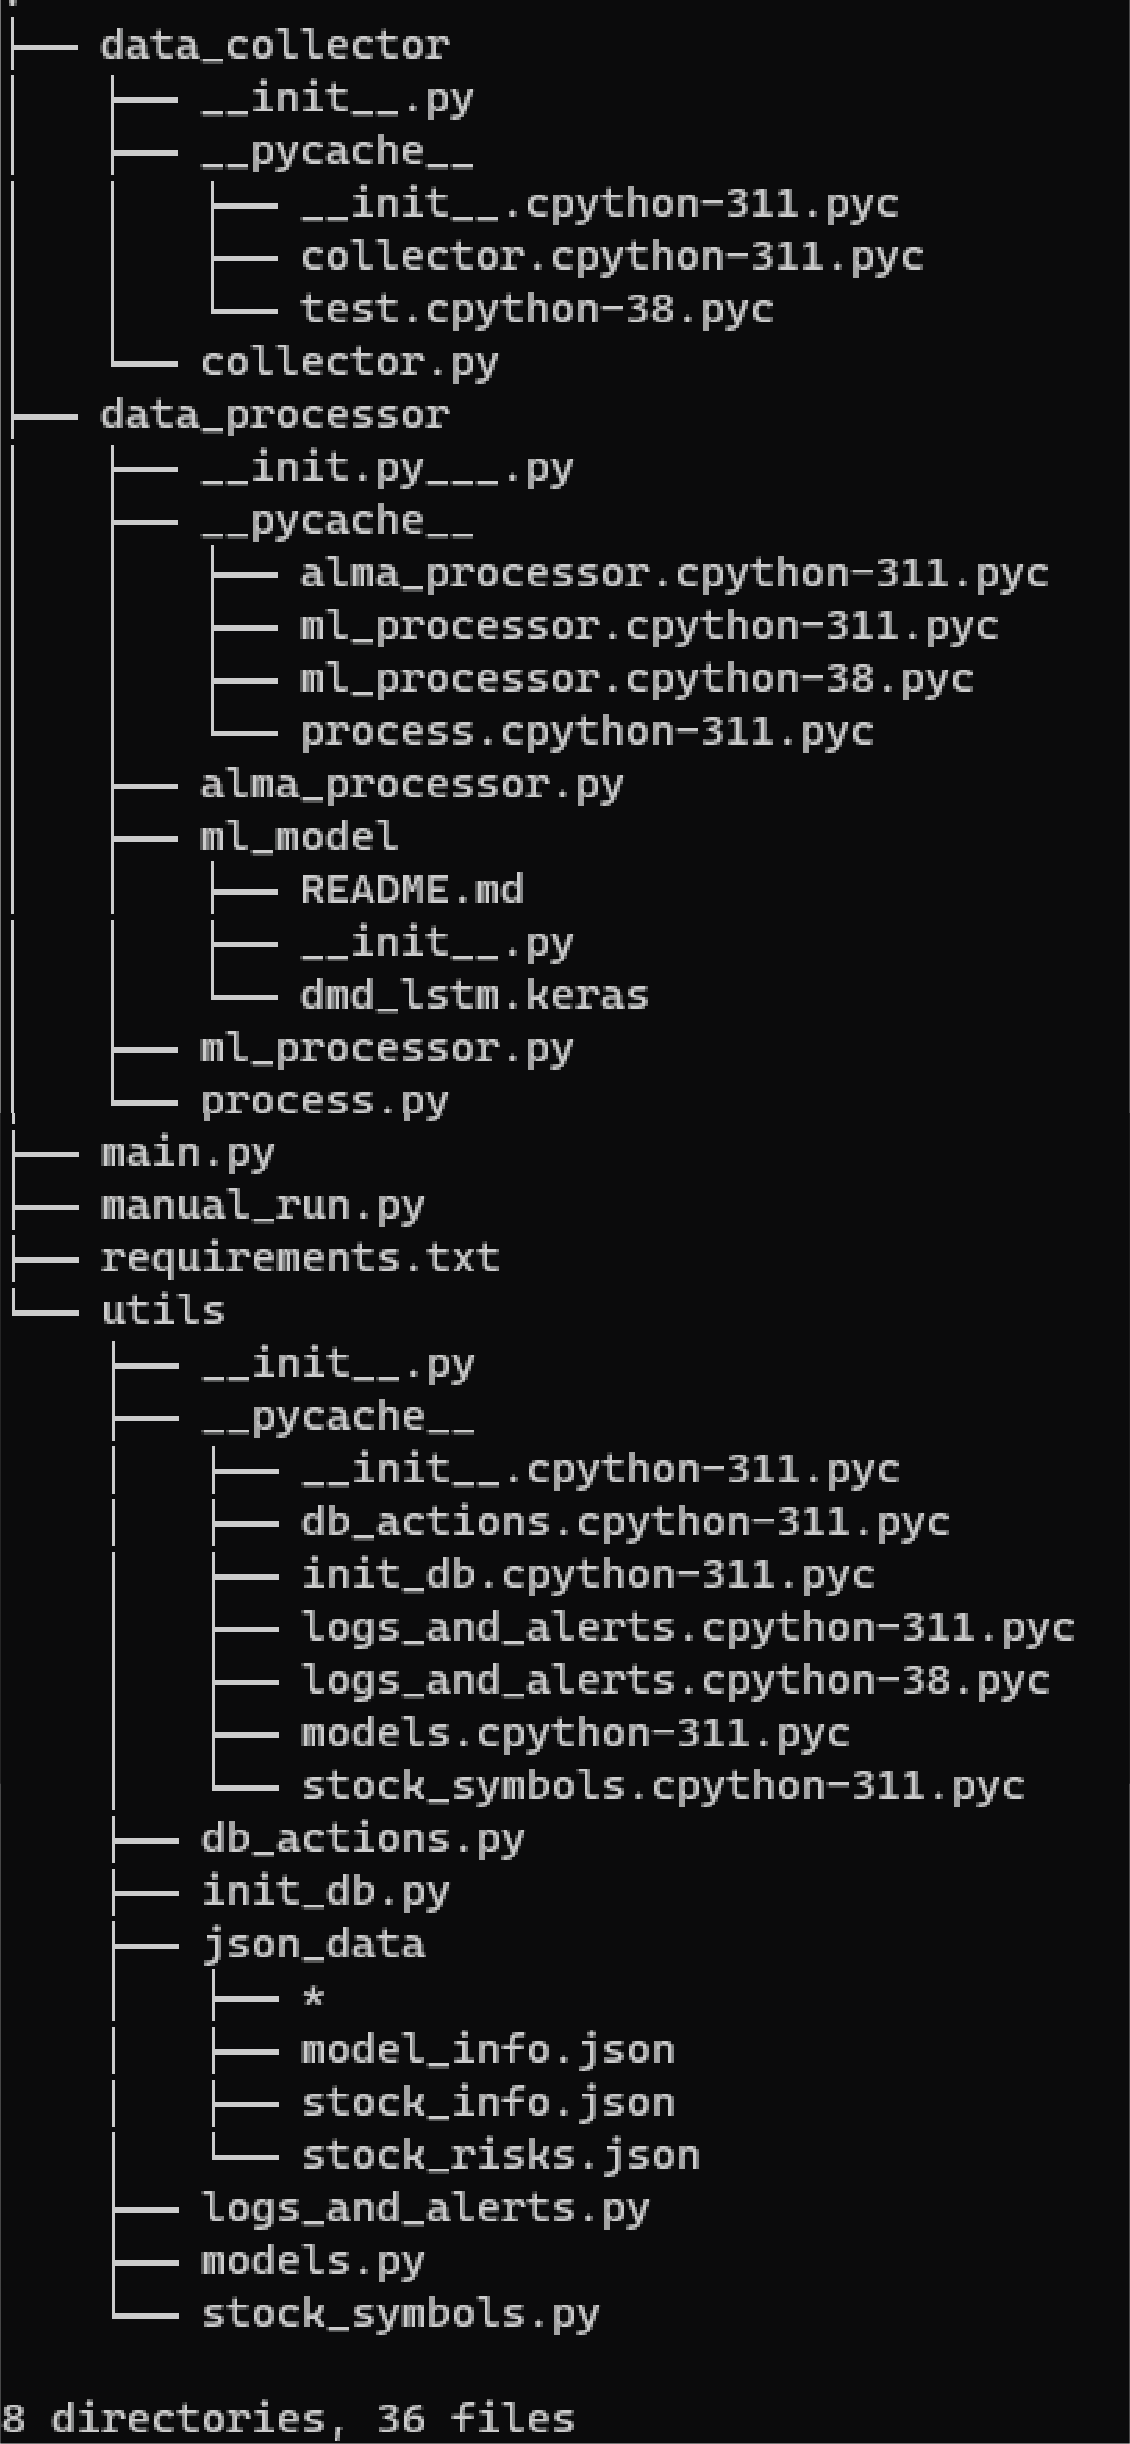
\includegraphics[height=0.60\textheight]{./assets/Chapter_4/Documentation/alampre_tree.png}
    \caption{alamPREPROCESSOR Docker Container Directory Tree}
    \label{fig:alampreproc_tree}
\end{figure}
\FloatBarrier

% Discuss /data/db volume (error logging and json_data directories)
On the other hand, the alamPREPROCESSOR shares the following directory paths related to error 
logging and json directories with the other components of the alamSYS via the '/data/db' directory path:
\begin{itemize}
    \item[(a)] /data\_collector\_logs - this is the directory for all the successful operations ('/success\_log.csv')
    , and all the unsuccessful operations ('/error\_log.csv') conducted by the data collector.
    \item[(b)] /data\_processor\_logs - this is the directory for all the successful operations ('/success\_log.csv')
    , and all the unsuccessful operations ('/error\_log.csv') conducted by the data processor.
    \item[(c)] /manual\_run\_logs - this is the directory for all the successful operations ('/success\_log.csv')
    , and all the unsuccessful operations ('/error\_log.csv') conducted by manually running the operations of the 
    alamPREPROCESSOR using the command 'python3 manual\_run.py'.
    \item[(d)] /preprocessor\_utils\_logs - this is the directory for all the logged actions conducted by utilities of alamPREPROCESSOR. 
    This is further divided into two directories, which are as follows:
    \begin{itemize}
        \item[1.] db\_actions - stores logs of successful operations ('/success\_log.csv'), 
        and all the unsuccessful operations ('/error\_log.csv') from the utilities related
        to database actions.
        \item[2.] init\_db - stores logs of successful operations ('/success\_log.csv')
        , and all the unsuccessful operations ('/error\_log.csv') from the utilities related
        to the initialization of the database.
    \end{itemize}
    \item[(f)] /scheduled\_task\_logs - this is the directory for all the successful operations ('/success\_log.csv')
    , and all the unsuccessful operations ('/error\_log.csv') conducted by the scheduled operation of the alamPREPROCESSOR.
\end{itemize}